\documentclass[border=10pt]{standalone}
\usepackage{tikz}
\usepackage{amsmath}
\usetikzlibrary{arrows.meta, positioning, fit, backgrounds, calc}

\begin{document}
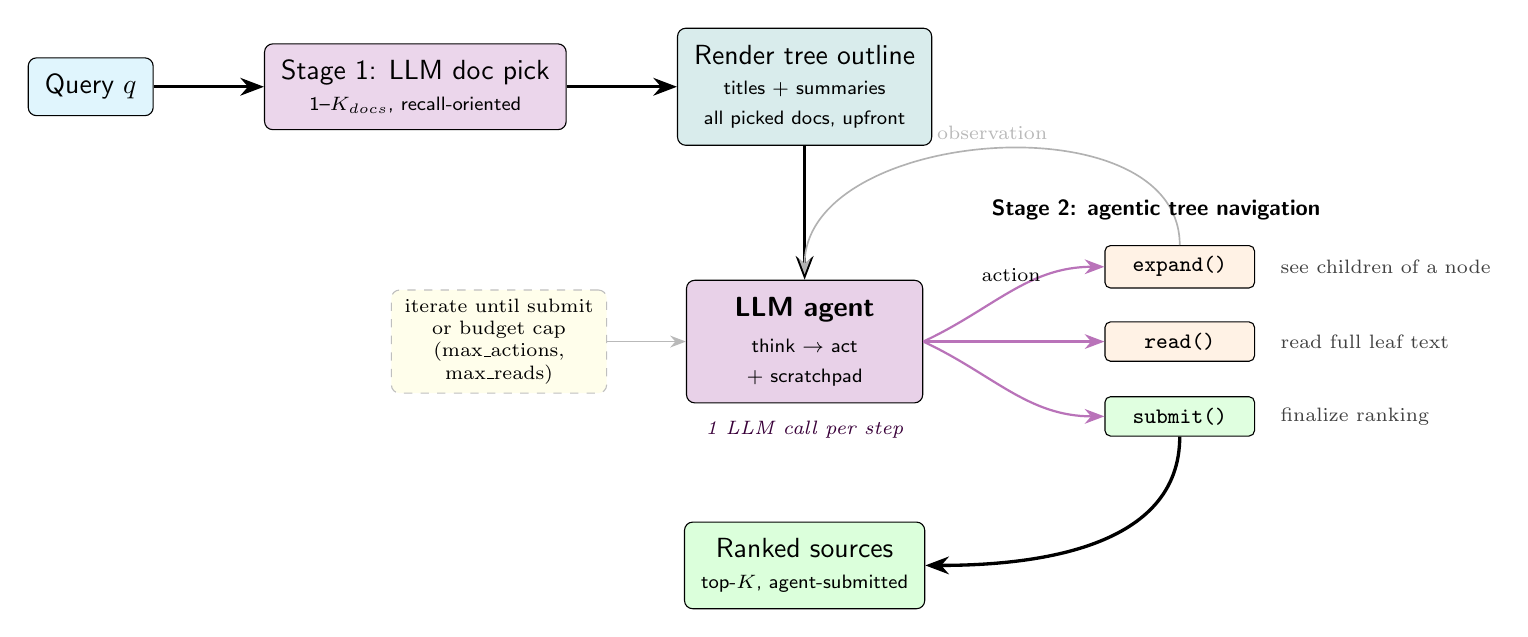
\begin{tikzpicture}[
    font=\small,
    box/.style={draw, rounded corners=3pt, align=center, font=\sffamily,
                inner sep=6pt},
    tool/.style={draw, rounded corners=2pt, align=center, font=\footnotesize\ttfamily,
                 inner sep=4pt, minimum width=1.9cm, fill=orange!10},
    flow/.style={-{Stealth[length=3mm]}, very thick},
    arr/.style={-{Stealth[length=2mm]}, semithick},
    loop/.style={-{Stealth[length=2.5mm]}, thick, violet!55},
]

    %==================== QUERY ====================
    \node[box, fill=cyan!12] (q) {Query $q$};

    %==================== STAGE 1: LLM doc pick ====================
    \node[box, fill=violet!16, right=1.4cm of q, align=center] (docpick)
        {Stage 1: LLM doc pick\\[-1pt]{\scriptsize 1--$K_{docs}$, recall-oriented}};
    \draw[flow] (q) -- (docpick);

    %==================== outline render ====================
    \node[box, fill=teal!15, right=1.4cm of docpick, align=center] (outline)
        {Render tree outline\\[-1pt]{\scriptsize titles $+$ summaries}\\[-1pt]
         {\scriptsize all picked docs, upfront}};
    \draw[flow] (docpick) -- (outline);

    %==================== AGENT (LLM) ====================
    \node[box, fill=violet!18, below=1.7cm of outline, align=center, minimum width=3.0cm,
          minimum height=1.3cm] (agent)
        {\textbf{LLM agent}\\[1pt]{\scriptsize think $\rightarrow$ act}\\[-1pt]
         {\scriptsize $+$ scratchpad}};
    \draw[flow] (outline) -- (agent);

    %==================== TOOLS (acted upon, observations returned) ====================
    \node[tool, right=2.3cm of agent, yshift=0.95cm] (expand) {expand()};
    \node[tool, right=2.3cm of agent] (read) {read()};
    \node[tool, fill=green!12, right=2.3cm of agent, yshift=-0.95cm] (submit) {submit()};

    % action arrows (agent -> tools)
    \draw[loop] (agent.east) to[out=25, in=180] node[above, font=\scriptsize, black]
        {action} (expand.west);
    \draw[loop] (agent.east) to[out=0, in=180] (read.west);
    \draw[loop] (agent.east) to[out=-25, in=180] (submit.west);

    % observation arrows back (expand/read -> agent) as one clear feedback path
    \draw[arr, gray!60, semithick] (expand.north) to[out=90, in=90]
        node[above, font=\scriptsize, gray!55, pos=0.5] {observation} ([yshift=2pt]agent.north);

    %==================== tool descriptions ====================
    \node[font=\scriptsize, text=gray!50!black, right=0.2cm of expand, align=left]
        {see children of a node};
    \node[font=\scriptsize, text=gray!50!black, right=0.2cm of read, align=left]
        {read full leaf text};
    \node[font=\scriptsize, text=gray!50!black, right=0.2cm of submit, align=left]
        {finalize ranking};

    %==================== budget / loop note ====================
    \node[draw=gray!50, dashed, rounded corners=3pt, fill=yellow!8, font=\scriptsize,
          align=center, left=1.0cm of agent, text width=2.5cm] (budget)
        {iterate until submit\\ or budget cap\\ (max\_actions,\\ max\_reads)};
    \draw[arr, gray!55] (budget.east) -- (agent.west);

    \node[font=\scriptsize\itshape, text=violet!45!black, below=0.1cm of agent]
        {1 LLM call per step};

    %==================== OUTPUT ====================
    \node[box, fill=green!14, below=1.5cm of agent, align=center] (out)
        {Ranked sources\\[-1pt]{\scriptsize top-$K$, agent-submitted}};
    \draw[flow] (submit.south) to[out=-90, in=0] (out.east);

    %==================== loop emphasis label ====================
    \node[font=\sffamily\bfseries\footnotesize, above=0.2cm of expand, xshift=-0.3cm]
        {Stage 2: agentic tree navigation};

\end{tikzpicture}
\end{document}